\chapter{Examples and Non-examples}

In this chapter, we will discuss the necessity of some of the restrictive assumptions made previously and explore the Einstein relation by examining some examples and -- by doing so -- will motivate some of the more general results of the next chapter.

\section{Euclidean Space}

We start by examining the classical setting of paragraph 1.2.1 in greater detail: Let once again $U\ssq\IR^n$ be an open, bounded, non-empty domain, equipped with Euclidean metric and $n$-dimensional Lebesgue-measure $\gl^n$. Trivially, $\dimh(U)=n$. 

For the Dirichlet-Laplace operator as introduced earlier, we obtain 
$\dims(U,-\gD)=\frac{n}{2}$ due to \eqref{eq:DECF}-\eqref{eq:dims}. Simultaneously, it is well-known that $\frac{1}{2}\gD$ is the generator of the $n$-dimensional Brownian motion $B_t$, which can easily be seen as follows:

By \eqref{eq:MPtoOp}, the semigroup $(T_t)_{t\geq0}$ induced by $B_t$ reads
\[
  T_tf(x)
   =\PTEp{f(B_t)}{x}
   =\frac{1}{(2\pi t)^{n/2}}\int_{\IR^n} 
     \exp\left(-\frac{|x-y|^2}{2t}\right)f(y)\,\Di y,
  \ f\in L^2(\IR^n,\gl^n)\cap C_c(E),
\]
Comparing this expression to the well-known convolution formula (see \cite[p.47]{evans2010partial})
\[
  u(x,t)=\frac{1}{(4\pi t)^{n/2}}\int_{\IR^n} \exp\left(-\frac{|x-y|^2}{4t}\right)f(y)\,\Di y,\ x\in\IR^n, t\geq0,
\]
for the solution of the heat equation $\gD u=\partial_t u$ on $\IR^n$ with initial value $u(x,0)=f(x)$, we can quickly derive that $\gD T_tf(x)=2\partial_t T_tf(x)$. Since imposing the Dirichlet boundary conditions on $\gD$ corresponds to killing $B_t$ at the boundary of $U$, we thus obtain by definition \ref{def:semigroup} the generator
\[
  Af=\frac{1}{2}\gD f,
\]
extended to its maximal domain $H_0^1(U,\mu)$. We conclude that the Markov process associated with $\gD$ is $2B_t$.

It remains to determine the walk dimension of the $n$-dimensional Brownian motion. This can be done in several ways, for example by appealing to Brownian scaling or by invoking Dynkin's formula after a standard truncation argument: By applying \cite[Lemma 19.21]{kallenberg2002foundations} to the function $u_x(y)=\frac{1}{2}|y-x|^2$, we get
\[
  \PTEp{\tau(r)}{x}
  =\PTEp{\int_0^{\tau(r)}\gD u_x(2B_s)\,\Di s}{x}
  =\PTEp{u_x\left(2B_{\tau(r)}\right)-u_x(0)}{x}
  =\PTEp{\frac{2r^2}{n}}{x}
  =\frac{2r^2}{n}
\]
Therefore, by definition \ref{def:dimw}, we obtain $\dimw(U,2B_t)=2$ which implies together with the results obtained previously that the Einstein relation (with constant 1) holds on $U$. 



\section{The Sierpinski Gasket}

\begin{figure}[h]
\centering
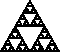
\includegraphics[scale=7]{sg.pdf}
\caption{An approximation of $\SG$}\label{fig:sg}
\end{figure}
The Sierpinski Gasket is a simple example of an iterated function fractal and can be described according to theorem \ref{thm:hutchinson} as the unique non-empty compact set $\SG\ssq\IR^2$ which is invariant under the three similitudes 
\[
  S_1(x,y)=\left(\frac{x}{2},\frac{y}{2}\right),\ 
  S_2(x,y)=\left(\frac{x+1}{2},\frac{y}{2}\right),\ 
  S_3(x,y)=\left(\frac{2x+1}{4},\frac{2y+\sqrt{3}}{4}\right),
\]
see figure \ref{fig:sg}. Since $\SG$ satisfies the (OSC), e.g. by taking the open equilateral triangle with corners $(0,0), (0,1)$ and $(1/2,\sqrt{3}/2)$, we obtain both 
\begin{equation}\label{eq:SGdimh}
  s=\dimh(\SG)=\frac{\ln 3}{\ln 2}
\end{equation}
and $\cH^s(\SG)\in(0,\infty)$ by a second appeal to Hutchinson's theorem. 

We will use the remainder of this section to establish the validity of the Einstein relation on $\SG$ with respect to the standard Laplace operator on $\SG$, which can be obtained in two different ways. In order to describe these constructions, we first need to fix some notation. 

Let $\scS=\{S_1,S_2,S_3\}$ as in section 1.1, set $\gS=\{1,2,3\}$ and denote by 
\[
  \gS^*:=\{\gep\}\cup\bigcup_{n\geq 1}\gS^n
\]
the free monoid consisting of all finite words over the alphabet $\gS$, where the monoid operation is given by concatenation and $\gep$ is supposed to represent the empty word. Using the monoid isomorphism 
$\gS^*\cong (\scS^*,\circ)$ given by extending 
$\gS\ni i\mapsto S_i\in\scS$, we can identify a word of length $l$,
\[
  w=w_1...w_l\in\gS^l,
\]
with the composition 
\[
  S_w:=S_{w_1}\circ...\circ S_{w_l}.
\]
By abuse of notation, we will therefore write $w(x)$ instead of $S_w(x)$. By an $n$-cell we understand the set $w(\SG)\ssq\SG$, where $w$ is a word of length $n$. Note that two different cells are either disjoint, or intersect in a single point which we will then call conjunction point, or one of them is completely contained in the other one. 

It is possible to approximate $\SG$ by a sequence of graphs $G_n$. Those graphs can be thought of as planar graphs with a triangle for each $n$-cell, where the vertices are the conjunction points between them. More precisely, let $G_n$ be the graph embedded in $\IR^2$ with vertex set $V_n$ inductively defined by
\begin{align*}
  V_0&:=
  \left\{(0,0),(0,1),\left(\frac{1}{2},\frac{\sqrt{3}}{2}\right)\right\}\\
  V_{n+1}&:=(S_1\cup S_2\cup S_3)(V_n),\ \ n\geq0.
\end{align*}
Additionally, set 
\[
  V*:=\bigcup_{n\geq0} V_n.
\]
Note that $V_0\ssq V_1\ssq...\ssq V_n\ssq ...$ and that
\[
  V_n=\bigcup_{w\in\gS^n} w(V_0).
\]
It also follows from the proof of Hutchinson's theorem that 
$d_H(V_n,\SG)\to 0$ as $n\to\infty$, so indeed, the graphs $G_n$ approximate $\SG$. 

\begin{figure}[h]
\centering
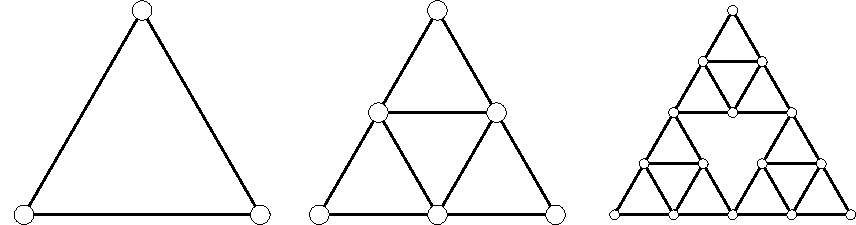
\includegraphics[scale=1]{gn.pdf}
\caption{The graphs $G_0,G_1,G_2$}\label{fig:gn}
\end{figure}

In $G_n$, connect two vertices $x,y\in V_n$ by a straight edge $xy$ iff they belong to the same $n$-cell, cf. figure \ref{fig:gn}, in which case we will call them neighbours and write $x\sim_n y$. By $E_n$ we mean the set of all edges in $G_n$. 



\subsection[Approximation by Dirichlet forms]{Approximation by Dirichlet forms\protect\footnote{The material in this section is an overview of the construction given in \cite[chapter I]{strichartz2006differential}}}

This analytic approach works by establishing so-called energy forms on graphs $G_n$ -- these are graph-theoretic discretisations of the Dirichlet form attached to the Laplace operator. For $n\in\IN$, define a bilinear form $\tilde\cE_n$ on $L^2(V_n)\cong \IR^{\# V_n}$ by 
\[
  \tilde\cE_n(f,g):=\sum_{xy\in E_n}(f(x)-f(y))(g(x)-g(y)), 
  \ \ \ f,g\in L^2(V_n).
\]
It is easy to check that this defines a local Dirichlet form on $L^2(V_n)$. As we will see, these bilinear forms are compatible with each other after a suitable renormalisation. Starting from $\tilde\cE_0$, consider a function 
$u\in\IR^3\cong L^2(V_0)$. Under all possible extensions 
$\tilde u$ to $\IR^6\cong L^2(V_1)$, which function is the harmonic extension of $u$, i.e. minimises $\tilde\cE_1[\tilde u]$? 

\begin{figure}[h]
\centering
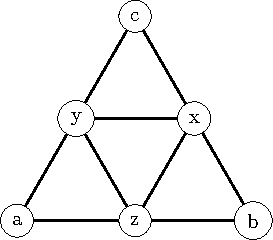
\includegraphics[scale=1]{g1.pdf}
\caption{The values of $u$ on $V_1$}\label{fig:g1}
\end{figure}

To answer this question, we label each vertex in $V_0$ by its value under $u$, say $a,b,c$ and each vertex in $V_1\setminus V_0$ by its value under $\tilde u$, say $x,y,z$ as in figure \ref{fig:g1}. Since we assume $u$ to be a fixed given function, the values $a,b,c$ are fixed, and we obtain 
\begin{multline}\label{eq:E1}
  \tilde\cE_1[\tilde u]=\left[(x-b)^2+(x-c)^2+(y-a)^2+(y-c)^2+(z-a)^2+(z-b)^2\right.\\
  \left.+(x-y)^2+(y-z)^2+(z-x)^2\right]
\end{multline}
Finding the minimising values for $x,y,z$ now becomes an exercise in multivariable calculus. Setting the partial derivatives equal to 0 yields the following system of linear equations:
\begin{align*}
  \begin{array}{c}
    8x=2(b+c+y+z)\\
    8y=2(a+c+x+z)\\
    8z=2(a+b+x+y)\\
  \end{array}\Longleftrightarrow
  \begin{array}{c}
    5x=a+2b+2c\\
    5y=2a+b+2c\\
    5z=2a+2b+c\\
  \end{array}
\end{align*}
Plugging this solution as $\tilde u$ in \eqref{eq:E1} to evaluate $\tilde\cE_1[\tilde u]$ gives
\begin{align*}
  \tilde\cE_1[\tilde u]
  &=\frac{1}{25}\left[(a-3b+2c)^2+(a+2b-3c)^2+(-3a+b+2c)^2
    +(2a+b-3c)^2\right.\\
  &\qquad\qquad \left.+(-3a+2b+c)^2+(2a-3b+c)^2
    +(b-a)^2+(c-b)^2+(a-c)^2\right]\\
  &=\frac{30}{25}\left[a^2+b^2+c^2-ab-ac-bc\right]\\
  &=\frac{3}{5}\tilde\cE_0[u]
\end{align*}
Using the fact that the vertices in $V_{n+1}\setminus V_n$ are in $G_n$ only adjacent to vertices in $V_n$ and that 
$\tilde\cE_{n+1}$ is local on $n$-cells it is possible to show by induction that each $u\in L^2(V_n)$ allows for a unique harmonic extension $\tilde u\in L^2(V_{n+1})$ and that 
\[
  \tilde\cE_{n+1}[\tilde u]=\frac{3}{5}\tilde\cE_n[u]
\]
for all $n\geq0$. This allows us to renormalise the bilinear form $\tilde\cE_n$ via 
\[
  \cE_{n+1}:=\left(\frac{3}{5}\right)^n\tilde\cE_n
\]
thus ensuring $\cE_{n+1}[\tilde u]=\cE_n[u]$ and therefore
$\cE_{n+1}[\hat u]\geq\cE_n[u]$ for any extension $\hat u$ of $u$.

Consider now any function $u:V^*\to\IR$ and denote its restriction to $V_n$ by $u_n$. Then, $\cE_n[u_n]$ is a nondecreasing sequence of nonnegative real numbers and therefore converges against 
\[
  \cE[u]:=\lim_{n\to\infty} \cE_n[u_n]\in[0,\infty].
\]
Define $\scD(\cE)$ to be the set of all functions $u:V^*\to\IR$ for which this limit is finite. It can be shown that $u\in\cE$ implies that $u$ is H\"older continuous and can therefore be uniquely extended to a continuous function on all of $\SG$. By abuse of notation we shall denote this extension by $u$ as well and set $\cE[u]:=\cE[u|_{V^*}]$ whenever the right-hand side is defined. Hence, by polarisation, we obtain a bilinear form $\cE(\cdot,\cdot)$ on $\scD(\cE)$. 

We further introduce the measure 
$\mu(\cdot):=\cH^s(\SG)^{-1}\cH^s(\cdot)$ on $\SG$. It is possible to show that the biliner form $(\cE,\scD(\cE))$ is a local regular Dirichlet form on $L^2(\SG,\mu)$ which in turn is attached to an operator as in equation \eqref{eq:DFtoOp}. This operator is what is known as standard Laplacian on $\SG$, and its spectral dimension is known to be $\frac{\log 3}{\log 5}$ (see e.g. \cite[section 3.5]{strichartz2006differential} or \cite{kigami1993weyl}). 

\subsection[Approximation by random walks]{Approximation by random walks\protect\footnote{The material in this section is an overview of the construction given in \cite[chapter II]{barlow1998diffusions}}}

It remains to discuss the walk dimension of the diffusion process generated by the standard Laplace operator on $\SG$. Once again, this construction uses the approximating graphs $G_n$. 

For $n\geq0$, let $Y^{(n)}_k, k\in\IN_0$ be a simple random walk on $G_n$, i.e. given $Y^{(n)}_k=v\in V_n$, the process has equal probability to jump to each of the neighbours of $v$ in $V_n$. 

Take $v\in V_{n-1}$. Then, $v$ is contained in either 1 or 2 $(n-1)$-cells with conjunction points 
$\{x_1,...,x_i\}\ssq V_n\setminus\{v\}$, $i\in\{2,4\}$ depending on whether or not $v\in V_0$. Assume $Y^{(n)}_0=v$, $n\geq1$. The only way for $Y^{(n)}$ to leave the $(n-1)$-cells containing $v$ is via the points $\{x_1,...,x_i\}$. However, due to the symmetry, the probabilities of hitting $x_j, j=1,...,i$ first are equal. If we set 
\begin{align*}
  T^{n,m}_0&=\inf\left\{t\in\IN_0:Y^{(n)}_t\in V_m\right\}\\
  T^{n,m}_{k+1} &=\inf\left\{t\in\IN_0, t>T^{n+1,m}_k:
     Y^{(n)}_t\in V_m\setminus \left\{Y^{(n)}_{T^{n,m}_k}\right\}\right\},\ \ k\geq0,
\end{align*}
for $n>m$, then $\left(Y^{(n)}_{T^{n,m}_k}\right)_{k\in\IN_0}$ is a standard random walk on $G_m$ and therefore equal to 
$\left(Y^{(m)}_k\right)_{k\in\IN_0}$ in distribution. Using self-similarity and standard arguments for finite Markov-chains, it can be shown that $\PTE{T^{n,m}_{k+1}-T^{n,m}_k}=5^{n-m}$ and that $Y^{(n)}$ overcomes a distance (in graph metric) of $2^{n-m}$. The renormalised processes $X^{(n)}_k:=Y^{(n)}_{5^nk}$, $k\in\IN_0$ furthermore converge almost surely and uniformly on compact intervals to a continuous limit process $(X_t)_{t\geq0}$ with values in $\SG$. Additionally, the infinitesimal generator of $X$ coincides with the $\SG$-Laplacian introduced above. 
By construction, this process possesses a self-similarity, in the sense that $(X_{5t})_{t\geq0}=(2X_t)_{t\geq0}$ in distribution for sufficiently small $t$, and it is not hard to show that $\dimw(\SG,X)=\frac{\log 5}{\log 2}$

Putting everything together, we obtain for the Sierpinski gasket:
\[
  \frac{\log 3}{\log 2}=\dimh(\SG)=\dims(\SG,\gD)\dimw(\SG,X)
  =\frac{\log 3}{\log 5}\frac{\log 5}{\log 2},
\]
so indeed, the Einstein relation holds on $\SG$.


\section{The real line as bounded metric space}


Bounded metric spaces form the most important class of spaces for which too naive of an adaption of \eqref{eq:defdimwrong} does not yield useful results. Indeed, consider the metric measure space 
$X=(\IR,d_{\arctan},\gl^1)$, where the metric is defined as $d_{\arctan}(x,y)=|\arctan(x)-\arctan(y)|$. Since 
\[
  \tan:\left(\left(-\frac{\pi}{2},\frac{\pi}{2}\right),|\cdot|\right)\to(\IR,d_{\arctan}) 
\]
provides an isometry, we have $\dimh(X)=1$. On this space, we consider the negative of the usual weak Laplace operator, $-\gD_{\gl^1}$, defined by mapping a function $u\in H_0^1(\IR,\gl^1)$ to the unique $g\in L^2(\IR,\gl^1)$ such that
\[
  \int_\IR g\gp\,\Di\gl^1=\int_\IR \partial_x u\partial_x \gp\,\Di\gl^1
\]
holds for all $\gp\in H_0^1(\IR,\gl^1)$. Notice how this does not differ from the negative weak Laplace operator on $(\IR,|\cdot|,\gl^1)$ since we did not change the measure and both metrics induce the same topology. Thus, we get from Weyl's classical result $\dims(X,-\gD_{\gl^1})=\frac{1}{2}$ and from the arguments developed in section 2.1 that the associated Markov process is $2(B_t)_{t\geq0}$. 

It is now easy to see that \eqref{eq:defdimwrong} does not provide a useful notion of a walk dimension: Since $B_{\arctan}(x,R)=\IR$ for every radius $R\geq\pi$, the expression diverges to $\infty$. Even the more careful approach 
\[
  \lim_{R\nearrow\frac{\pi}{2}}\frac{\log \PTEp{\tau(R)}{0}}{\log R}
\]
runs into similar problems: Using the formula $\PTE{\tau([a,b])}=-ab$ for the exit time of a standard Brownian motion from the intervall $[a,b]\ni 0$, we get
\[
  \log \PTEp{\tau(B_{\arctan}(0,R))}{0}=2\log \tan R =\infty.
\]
However, the local walk dimension from definition \ref{def:dimw} works out quite elgantly: Setting $y=\arctan x\in\left(-\frac{\pi}{2},\frac{\pi}{2}\right)$, we obtain for some $\xi_1\in (y,y+r),\xi_2\in(y-r,y)$
\begin{multline*}
  \frac{\log \PTEp{\tau\big(B_{\arctan}(0,R)\big)}{0}}{\log r}
  =\frac{\log\left(\tan(y+r)-\tan y\right)}{\log r}+\frac{\log\left(\tan y-\tan (y-r)\right)}{\log r}\\
  =\frac{\log\frac{r}{\cos^2 \xi_1}}{\log r}+\frac{\log\frac{r}{\cos^2 \xi_2}}{\log r}
  =2-\frac{\log \cos^2 \xi_1}{\log r}-\frac{\log\cos^2 \xi_2}{\log r}
\end{multline*}
by using the mean value theorem. Taking the limit for $r\searrow0$ on both sides implies $\xi_1,\xi_2\to y$ and thus $\dimw(E,2B_t,x)=2$. 







